Principal component analysis (PCA) is a coordinate transform that minimizes projection residuals along each of the major axes \(e_1, e_2, \dots, e_m\) of the transformed space.
These axes are referred to as \textbf{principal components}.
After the PCA transform is applied to a set of observations, the smallest projection error is along the first principal component.
If we project down to two dimensions, the first two principal components have the smallest projection error.
In general, projecting down to \(k \leq m\) dimensions is most accurate along \(e_1, e_2, \dots, e_k\).

Conversely, projecting along \(e_2, \dots, e_m\) will result in the largest residual error in \(m-1\) dimensions.
It follows that \(e_1\) must be the direction with the highest variance.
Then \(e_2\) is the direction with the next highest variance, and so on.
% In this way, we can picture PCA as the covariance ellipsoid for the original data.

\begin{example}
    \def\Amat{\begin{bmatrix}
        5 &  3 &  6 &  7 &  6 \\
        4 &  5 &  7 &  1 &  3 \\
        5 &  7 &  6 &  1 &  0 \\
        6 & 10 & 12 & 12 & 11 \\
        9 & 10 & 12 & 13 &  9 \\
    \end{bmatrix}}
    Consider the following matrix \[A = \Amat.\]
    The column means are \(\mu = [5.8,7,8.6,6.8,5.8]\).
    Then the mean-centered data becomes
    \def\-{\phantom{-}}
    \[X = A - \mu = \frac{1}{5}\begin{bmatrix}
            -4 &   -20 &   -13 &   \-1 &   \-1 \\
            -9 &   -10 &    -8 &   -29 &   -14 \\
            -4 &   \-0 &   -13 &   -29 &   -29 \\
            \-1 &  \-15 &  \-17 &  \-26 &  \-26 \\
        \-16 &  \-15 &  \-17 &  \-31 &  \-16 \\
    \end{bmatrix}.\]

    The covariance matrix is
    \[C = X^TX = \frac{1}{5}\begin{bmatrix}
            74 &  85 &  93 & 179 & 104 \\
            85 & 190 & 170 & 225 & 150 \\
            93 & 170 & 196 & 313 & 238 \\
        179 & 225 & 313 & 664 & 484 \\
        104 & 150 & 238 & 484 & 394 \\
    \end{bmatrix}.\]
    
    Diagonalizing \(C\) gives
    \begin{align*}
        V &= \begin{bmatrix}
            0.1888 & -0.2020 & -0.6366 &  0.5495 & -0.4651\\
            0.2755 & -0.7886 &  0.1472 & -0.4502 & -0.2791\\
            0.3606 & -0.3464 &  0.3128 &  0.5836 &  0.5582\\
            0.6979 &  0.2522 & -0.4422 & -0.3707 &  0.3411\\
            0.5209 &  0.3922 &  0.5288 &  0.1316 & -0.5271\\
        \end{bmatrix},\\
        D &= \begin{bmatrix}
            264.8458 &       0 &      0 &      0 & 0 \\
                    0 & 27.9766 &      0 &      0 & 0 \\
                    0 &       0 & 9.3198 &      0 & 0 \\
                    0 &       0 &      0 & 1.4579 & 0 \\
                    0 &       0 &      0 &      0 & 0 \\
        \end{bmatrix}.
    \end{align*}
    
    If we keep all \(5\) principal component vectors, then \(V_5 = V\) and the projection of \(X\) along \(V\) is
    \[P = XV = \begin{bmatrix}
        -1.9469 &  4.3453 & -0.8756 & -0.2039 & 0 \\
        -6.9742 & -0.0660 &  1.4352 &  0.7590 & 0 \\
        -8.1577 & -2.6752 & -0.8063 & -0.5704 & 0 \\
            8.4282 & -0.2330 &  1.8282 & -0.4996 & 0 \\
            8.6507 & -1.3711 & -1.5815 &  0.5149 & 0 \\
    \end{bmatrix}.\]
    Here, the last column of \(P\) is the zero vector because the last eigenvalue of \(C\) is zero\footnote{Since we subtracted the column means from a square matrix \(A\), the dimension of the row space was reduced to 4.}.
    To perfectly reconstruct \(A\), we need \(k = 4\) principal components and the row vector \(\mu\)
    \[A = PV^T + \mu = PV_4^T + \mu.\]
    
    If we use \(k = 3\) principal components, then the projection of \(X\) onto \(V_3\) is
    \[P = XV_3 = \begin{bmatrix}
        -1.9469 &  4.3453 & -0.8756 \\
        -6.9742 & -0.0660 &  1.4352 \\
        -8.1577 & -2.6752 & -0.8063 \\
            8.4282 & -0.2330 &  1.8282 \\
            8.6507 & -1.3711 & -1.5815 \\
    \end{bmatrix}\]
    and \(A\) is approximately reconstructed by
    \[A \approx P V_3^T + \mu = \begin{bmatrix}
        % 5.1121 &  2.9082 &  6.1190 &  6.9244 &  6.0268 \\
        % 3.5829 &  5.3417 &  6.5570 &  1.2814 &  2.9001 \\
        % 5.3134 &  6.7432 &  6.3329 &  0.7886 &  0.0751 \\
        % 6.2745 &  9.7751 & 12.2916 & 11.8148 & 11.0658 \\
        % 8.7170 & 10.2318 & 11.6995 & 13.1909 &  8.9322 \\
        5.1 &  2.9 &  6.1 &  6.9 &  6.0 \\
        3.6 &  5.3 &  6.6 &  1.3 &  2.9 \\
        5.3 &  6.7 &  6.3 &  0.8 &  0.1 \\
        6.3 &  9.8 & 12.3 & 11.8 & 11.1 \\
        8.7 & 10.2 & 11.7 & 13.2 &  8.9 \\
    \end{bmatrix}.\]
    We can compute the reconstruction error using
    \begin{equation*}%\label{eqn:reconstruction_error}
        E_k = \|A - (PV_k^T + \mu)\|_F,
    \end{equation*}
    where \(\|\cdot\|_F\) is the Frobenius norm.
    By the SVD, we have \(X = USV^T\), where \(S = \sqrt{D}\).
    So, the projection of \(X\) onto \(V_k\) is \[P = XV_k = US_k,\] where \(S_k\) is the diagonal matrix of the first \(k\) singular values.
    Then the reconstruction error becomes
    \begin{align*}
        \|A - (PV_k^T + \mu)\|_F
        &= \|(A - \mu) - PV_k^T\|_F \\
        &= \|X - PV_k^T\|_F \\
        &= \|USV^T - US_kV^T\|_F \\
        &= \|U(S - S_k)V^T\|_F \\
        &= \|S-S_k\|_F \\
        &= \sigma_k + \sigma_{k+1} + \dots + \sigma_{p}.
    \end{align*}
    Hence,
    \[E_3 = \sigma_3 + \sigma_4 = \sqrt{1.4579} + 0 = 1.2074.\]
\end{example}

\subsection{Ordinary least squares and PCA}
\def\vb#1{\mathbf{#1}}
Let \(X\) and \(Y\) be random variables corresponding to observation vectors \(\vb{x}\) and \(\vb{y}\).
Suppose we want to fit a linear model such that \(Y \sim 1 + X\).

In two dimensions, the model for ordinary least squares (OLS) regression reduces to
\def\cov{\operatorname{cov}}
\def\Var{\operatorname{var}}
\begin{equation}
    \label{eqn:ols-model}
    y(x) = \frac{\cov(\vb{x},\vb{y})}{\Var(\vb{x})}(x - \overline{\vb{x}}) + \overline{\vb{y}},
\end{equation}
This model minimizes the sum of squared errors when used to predict \(\vb{y}\) values.
If we model \(X\) as the target instead, OLS would yield a different formula.
In contrast, PCA can be used to create the regression model\footnote{I think this model would be considered total least squares (TLS) regression since it uses all variables (input and output). Principal component regression (PCR) creates the regression equation using only the input variables.}
\begin{equation}
    \label{eqn:pca-model}
    y(x) = \frac{\lambda_{\max} - \Var({\vb{x}})}{\cov(\vb{x},\vb{y})}(x - \overline{\vb{x}}) + \overline{\vb{y}},
\end{equation}
where \(\lambda_{\max}\) is the largest eigenvalue of the covariance matrix
\[\begin{bmatrix}
    \cov(\vb{x}, \vb{x}) & \cov(\vb{x}, \vb{y}) \\
    \cov(\vb{y}, \vb{x}) & \cov(\vb{y}, \vb{y})
\end{bmatrix} = \begin{bmatrix}
    \Var(\vb{x}) & \cov(\vb{x}, \vb{y}) \\
    \cov(\vb{x}, \vb{y}) & \Var(\vb{y})
\end{bmatrix}.\]
In particular,
\[\lambda_{\max} = \frac{1}{2}\left(\Var(\vb{x}) + \Var(\vb{y}) + \sqrt{(\Var(\vb{x}) - \Var(\vb{y}))^2 + 4\cov(\vb{x},\vb{y})^2}\right).\]
The PCA model minimizes orthogonal projection residuals, that is, the line given by \eqref{eqn:pca-model} results in the shortest total distance to the set of points \(\{(x^{(i)},y^{(i)})\}\).
So, whether \(X\) or \(Y\) is treated as the target variable, the regression line is the same.
See \Cref{fig:ols-pca}.

\begin{figure}
    \centering
    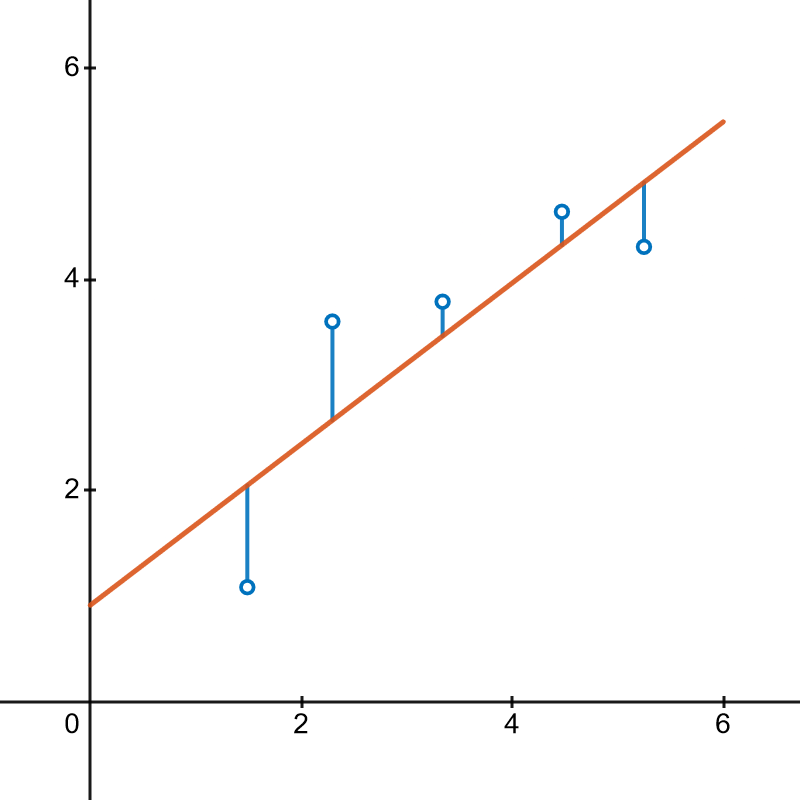
\includegraphics[width=.4\linewidth]{figs/fig-least-squares.png}
    \hfill
    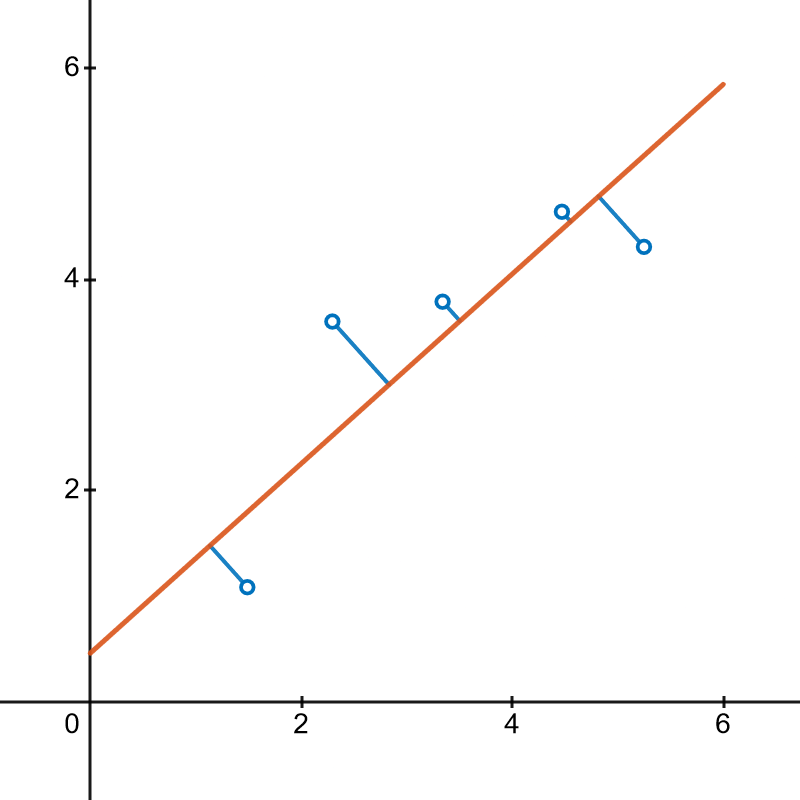
\includegraphics[width=.4\linewidth]{figs/fig-orthogonal-regression.png}
    \caption{Ordinary least squares (left) minimizes the sum of squared errors while total least squares, i.e., the PCA model (right) minimizes the orthogonal projections.}
    \label{fig:ols-pca}
\end{figure}